\section{Nonlinear Latent Variable Models}

  Now we will consider ourselves with nonlinear latent variables models. Recall that a latent variable model consists of an \textit{inference model} $p(z \mid x)$ that encodes the data in a latent space and a \textit{generative model} $p_\theta (x \mid z)$. Given the covariates $x$ we assume that they are generated by sampling from the simple latent distribution $p(z)$, called our \textit{prior}, and calculate 
  \begin{equation}
    p_\theta (x, z) = p_\theta (x \mid z) \, p(z)
  \end{equation}
  where $p_\theta (x \mid z)$ can be computed from our generative model. However, computing 
  \begin{equation}
    p_\theta (x) = \int p_\theta (x, z) \,dz = \int p_\theta (x \mid z) \, p(z) \,dz
  \end{equation}
  is computationally intractable, which means that taking the derivative of the log-likelihood is also impossible. 
  \begin{equation}
    \ell(\theta) = \sum_i \log p_\theta (x^{(i)})
  \end{equation}
  At first, it seems like all hope is lost, but statisticians have a few tricks up their sleeves. 
  \begin{enumerate}
    \item The first trick is called the variational lower bound, which is a lower bound on the log likelihood, and therefore by optimizing it we can hope to optimize the log-likelihood as well. This works well in practice. 
    \item The next trick is by optimizing the Fisher score, which is the gradient of the log likelihood \textit{with respect to the covariates} (not the parameters!). 
  \end{enumerate}

\subsection{Variational Lower Bounds and EM Algorithm} 

  To simplify the computation, we start off with the log likelihood for just one sample. 

  \begin{definition}[Evidence Lower Bound]
    To lower bound it, we can use Jensen's inequality\footnote{Given convex function $f: \mathbb{R} \rightarrow \mathbb{R}$, and random variable $X$, $\mathbb{E}[f(x)] \geq f(\mathbb{E}[X])$.} with the concave function $f(x) = \log(x)$ over domain $\mathbb{R}^+$ and the following holds true for all $\theta$ and more importantly, for \textit{any arbitrary density function} $q(z)$. Therefore, we have 
    \begin{align}
      \ell(\theta) & = \log p_\theta (x) \\
                   & = \log \int p_\theta (x \mid z) \, p(z) \,dz \\
                   & = \log \int q(z) \frac{p_\theta (x \mid z) \, p(z)}{q(z)} \,dz \\ 
                   & \geq \int q(z) \log \bigg( \frac{p_\theta (x \mid z) \, p(z)}{q(z)} \bigg) \,dz \\  
                   & = \elbo_{q, \theta}(x) 
    \end{align}
    The lower bound is called the \textbf{evidence lower bound (ELBO)}, or \textbf{variational lower bound}. 
  \end{definition} 

  So every density $q$ will give a different lower bound, which is why this is \textit{variational}. Why is this necessarily simpler to calculate? 


  Suppose we have an estimation problem given the training set $\{x^{(i)}\}_{i=1}^n$. We have latent variable model $p(x, z; \theta)$ with $z$ being the latent variable of discrete, finite random variable $Z$, with density $p_Z (z)$. Let us denote the density of $X$ as $p_X$. Then, the random variable $X$ can be interpreted as us first generating $z$ from $Z$, and then computing $X\,|\,Z = z$.  
  \[\text{Compute } X = \text{Compute } Z \text{ and then } \begin{cases} 
  \text{Compute } X \,|\, Z = 1 \\
  \text{Compute } X \,|\, Z = 2 \\
  \ldots \\
  \text{Compute } X \,|\, Z = k
  \end{cases}\]

  Let us clarify some notation: 
  \begin{itemize}
    \item The distribution that we will iteratively reassign over and over again is $Z$, with density $p_Z$ that maps $z \mapsto \phi_z$, where $\phi$ is a vector that represents the density.
    \item The $k$ conditional (not necessarily Gaussian) distributions that we will iteratively reassign over and over again is $X_1, X_2, \ldots, X_k$, with densities $p_{X_1} (x), \ldots, p_{X_k} (x)$ that maps $x \mapsto p_{X_j} (x)$.
    \item The distribution of the entire random variable $X$ will have density $p_X (x)$. Since we are iteratively reassigning the densities $p_Z$ and $p_{X_j}$, this joint distribution of $X$ will also get modified.
  \end{itemize}

  The EM algorithm in the general case has the following steps: 
  \begin{enumerate}
    \item We initialize the value of $\theta$ in some way. Note that within this $\theta$ are the parametizations of the initial multinomial density $p_Z$, which is our initial "guess" of the distribution of $Z$.
    \item \textbf{(E Step)} The log likelihood of the given data $\{ x^{(i)}\}_{i=1}^n$ with respect to the parameter $\theta$ (which encodes all parameters of distribution $Z$ and all $X\,|\,Z$) is 
      \[l(\theta) = \sum_{i=1}^n \log\, p_X \big( x^{(i)}; \, \theta \big)\]
    It turns out that explicitly finding the maximum likelihood estimates of the parameters $\theta$ is hard because it results in a difficult, non-convex optimization problem. So, we tackle this another way. 
    
    To start, we can see that the summation isn't too crucial, so we can focus on minimizing each $\log \, p_X \big(x^{(i)}; \, \theta \big)$ and summing in the end. We can calculate this by conditioning over all $j = 1, \ldots, k$ generated from $Z$ (which we have guessed to have an initial density of $p_Z$). That is, we must find for each $i = 1, 2, \ldots, n$ 
    \begin{align*} 
      \max_\theta \log \, p_X \big( x^{(i)}; \, \theta \big) & = \max_\theta \log \, \bigg(\sum_{j=1}^k p_X \big(x^{(i)}, Z = j; \, \theta\big) \bigg) \\
      & = \max_\theta \log \bigg( \sum_{j=1}^k p_X \big( x^{(i)}\,|\, Z = j; \, \theta\big) p_Z \big( j; \, \theta \big) \bigg) \\
      & = \max_\theta \log \bigg( \sum_{j=1}^k p_{X_j} \big( x^{(i)} ;\, \theta\big) p_Z \big( j; \, \theta \big) \bigg)
    \end{align*}
    To find this maximum value, we can focus on the first equality and see that by Jensen's inequality (with conCAVE, not convex, $f(x) = \log x$ over domain $x \in \mathbb{R}^+$), the following holds true for all $\theta$ and more importantly, for \textit{any arbitrary density function} $p_Z^{*i}$.  
    \begin{align*} 
      \log p_X \big(x^{(i)};\, \theta\big) & = \log \bigg( \sum_{j=1}^k p_X \big(x^{(i)}, Z = j;\, \theta \big) \bigg) \\ 
      & = \log \bigg( \sum_{j=1}^k p_Z^{*i} \big(j \big)\, \frac{p_X \big(x^{(i)}, Z = j;\, \theta \big)}{p_Z^{*i} \big(j \big)} \bigg) \\
      & = \log \Bigg(\mathbb{E}_{j \sim p_Z^{*i}} \bigg( \frac{p(x^{(i)}, Z = j; \, \theta)}{p_Z^{*i} \big(j \big)}\bigg)\Bigg) \\
      & \geq \mathbb{E}_{j \sim p_Z^{*i}} \Bigg( \log \bigg( \frac{p(x^{(i)}, Z = j; \, \theta)}{p_Z^{*i} \big(j \big)} \bigg) \Bigg) \\
      & = \sum_{j=1}^k p_Z^{*i} (j) \, \log\bigg( \frac{p(x^{(i)}, Z = j; \, \theta)}{p_Z^{*i} (j)} \bigg) = \text{ELBO} \big( x^{(i)}; \,p_Z^{*i}, \theta \big)
    \end{align*}
    The final term, called the \textbf{evidence lower bound} (ELBO), is just the expectation of $\log \frac{p(x^{(i)}, Z = j; \, \theta)}{p_Z^{*i} (j)}$ with respect to $j$ drawn from density $p_Z^{*i}$, which is denoted with $\mathbb{E}_{j \sim p_Z^{*i}}$. 
    
    Summing over all $n$ examples, we have a lower bound for the entire log likelihood for \textit{any} set of density functions $p_Z^{*1}, p_Z^{*2}, \ldots, p_Z^{*n}$: 
    \begin{align*} 
      l(\theta) = \sum_{i=1}^n \log p(x^{(i)}; \, \theta) & \geq \sum_{i=1}^n \text{ELBO}(x^{(i)}; \, p_Z^{*i}, \theta) \\
      & = \sum_{i=1}^n \sum_{j=1}^k p_Z^{*i} (j) \, \log\bigg( \frac{p(x^{(i)}, Z = j; \, \theta)}{p_Z^{*i} (j)} \bigg)
    \end{align*}
    Our job now is to choose the correct density functions $p_Z^{*i}$'s such that the lower bound is maximized. It turns out that we can do even better: equality is satisfied if and only if we set 
    \begin{align*} 
      p_Z^{*i} (j) & \equiv p_Z \big( j\,|\, x^{(i)}; \, \theta \big) \\
      & \equiv p_Z^{(i)} \big( j; \, \theta \big) \text{ for all } i = 1, 2, \ldots, n
    \end{align*}
    which is simply the posterior distribution of the multinomial given the observed sample $x^{(i)}$, which we can easily calculate using Bayes' rule. Substituting this into $p_Z^{*i}$ leads to the equality 
    \begin{align*} 
      l(\theta) = \sum_{i=1}^n \log p (x^{(i)}; \, \theta) 
      & = \sum_{i=1}^n \text{ELBO}\big(x^{(i)}; p_Z^{(i)}, \, \theta \big) \\
      & = \sum_{i=1}^n \sum_{j=1}^k p_Z^{(i)} \big( j; \, \theta \big) \, \log\bigg( \frac{p(x^{(i)}, Z = j; \, \theta)}{p_Z^{(i)} \big( j; \, \theta \big)} \bigg) \\
      & = \sum_{i=1}^n \sum_{j=1}^k p_Z \big( j\,|\, x^{(i)}; \, \theta \big) \, \log\bigg( \frac{p(x^{(i)}, Z = j; \, \theta)}{p_Z \big( j\,|\, x^{(i)}; \, \theta \big)} \bigg)
    \end{align*}
    In summary, this E step has taken the log-likelihood function $l(\theta)$ (representing (the log of) the probability of all the $x^{(i)}$'s landing where they are given the parameters $\theta$), which is abstract and hard-to-optimize, and converted it into an equivalent form as the sum of a bunch of ELBO functions optimized with the density parameters begin assigned $p_Z^{*i} = p_Z^{(i)}$. 
    
    But remember that these optimal densities $p_Z^{*i} = p_Z^{(i)}$ make the right and left hand side equivalent only for a \textbf{fixed value} of $\theta$! So, the right hand side is only equivalent to $l(\theta)$ only for that one value of $\theta$, but as soon as we set $\theta$ to something else, the right hand side evaluated with $p_Z^{*i} = p_Z^{(i)}$ are not equal.
    \item \textbf{(M Step)} Since we have found some equivalent form of $l(\theta)$ for the fixed $\theta$ that was initialized, we can now just maximize the right hand side with respect to $\theta$, while fixing the $p_Z^{*i} = p_Z^{(i)}$'s. Therefore, we find and set the value of $\theta$ as 
    \begin{align*}  
      \theta & = \text{arg}\; \max_\theta \sum_{i=1}^n \text{ELBO} \big( x^{(i)}; \, p_Z^{(i)}, \theta \big) \\
      & = \text{arg}\; \max_\theta \sum_{i=1}^n \sum_{j=1}^k p_Z^{(i)} (j)\; \log \bigg( \frac{p(x^{(i)}, Z = j; \, \theta)}{p_Z^{(i)} (j)} \bigg) \\
      & = \text{arg}\; \max_\theta \sum_{i=1}^n \sum_{j = 1}^k p_Z \big(j\,|\, x^{(i)}; \, \theta \big)\, \log \bigg( \frac{p(x^{(i)}, Z = j; \, \theta)}{p_Z \big(j\,|\, x^{(i)}; \, \theta \big)} \bigg)
    \end{align*}
    In the case where the parameter $\theta$ consist of $\phi, \mu_1, \ldots, \mu_k, \Sigma_1, \ldots, \Sigma_k$ like in the GMM model, it happens so that the maximum is found by computing $\phi$ to be the average of the $\phi^{(i)}$'s, each $\mu_j$ to be the weighed averages of the points, and each $\Sigma_j$ as the equation above. For other distributions, the formula for the maximum must be mathematically found (or algorithmically computed) with respect to parameter $\theta$.
    \item We have now reassigned the entire value of $\theta$, meaning that the parameters representing our guess of density $p_Z$ of $Z$ has also been modified. With this new value of $\theta$, we repeat steps 2 and 3 until convergence.
  \end{enumerate}

  For some intuition, we can visualize $l$ as a function of $\theta$. For the sake of visuals, we will assume that $\theta \in \mathbb{R}$ and $l: \mathbb{R} \longrightarrow \mathbb{R}$. On the contrary to what a visual is supposed to do, we want to point out that we cannot just visualize $l$ as a curve in $\mathbb{R} \times \mathbb{R}$. This can be misleading since then it implies that the optimal $\theta$ value is easy to find, as shown in the left. Rather, we have no clue what the whole curve of $l$ looks like, but we can get little snippets (right). 

  \begin{figure}[H]
    \centering 
    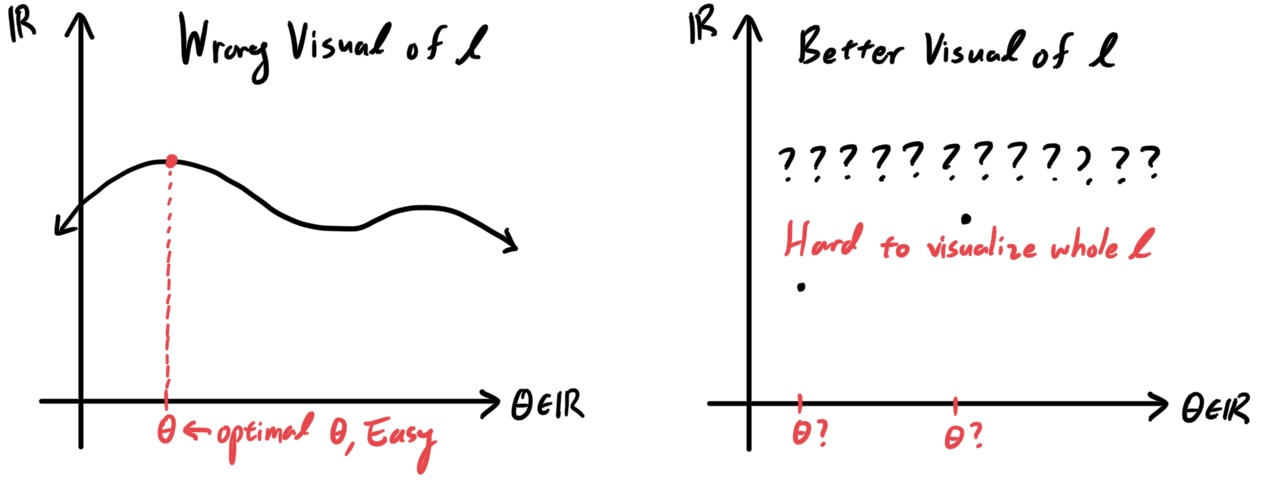
\includegraphics[width=0.6\textwidth]{img/visual_of_l.jpg}
    \caption{} 
    \label{fig:visual_of_l}
  \end{figure}

  Rather, all we can do is hope to take whatever easier-to-visualize, lower-bound functions and maximize them as much as we can in hopes of converging onto $l$. Let us walk through the first two iterations of the EM algorithm. We first initialize $\theta$ to, say $\theta_0$. This immediately induces the lower-bound ELBO-sum function $\sum_{i} \text{ELBO} (x^{(i)};\, p_Z^{*i}, \theta)$, which takes in multinomial density functions $p_Z^{*i} = p_1, p_2, \ldots$ and outputs different functions of $\theta$ that are valid lower bounds. Two of these possible lower-bound functions are shown (in green) for when we input some arbitrary density $p_1, p_2$. However, there exists a density $p_Z^{(i)}$ that produces not only the maximum possible lower-bound (called max ELBO, shown in red) but is equal to $l(\theta)$ for that density input $p_Z^{(i)}$. We maximize this function with respect to $\theta$ to get $\theta_1$ as our next assignment of $\theta$. 

  \begin{figure}[H]
    \centering 
    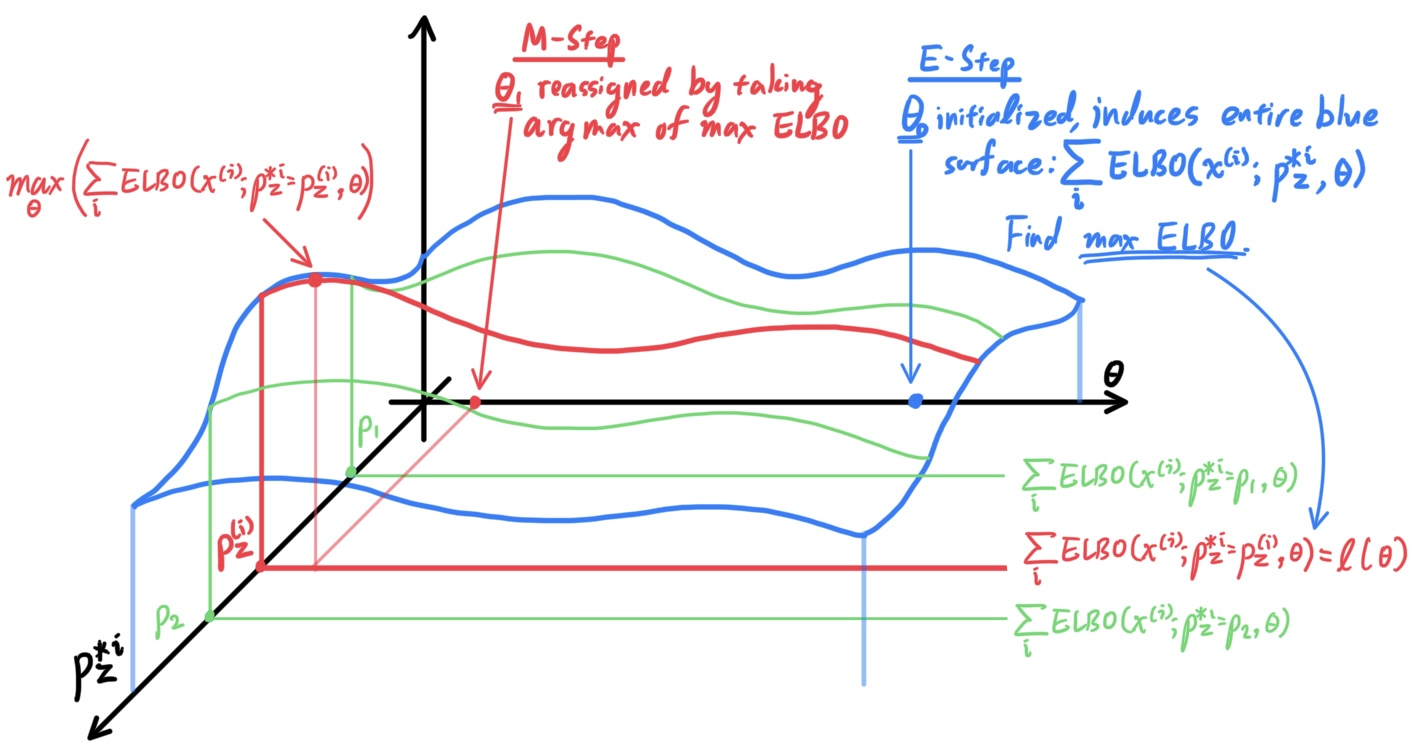
\includegraphics[width=0.7\textwidth]{img/EM_first_iteration.jpg}
    \caption{} 
    \label{fig:EM_first_iteration}
  \end{figure}

  The next step is identical. Now that we have a new value of $\theta = \theta_1$, this induces the lower-bound ELBO-sum function $\sum_{i} \text{ELBO} (x^{(i)};\, p_Z^{*i}, \theta)$ that also takes in multinomial densities $p_Z^{*i}$ and outputs different functions of $\theta$ that are valid lower-bounds. Two possible lower bounds are shown (in green), but the maximum lower-bound (in blue) is produced when we input density $p_Z^{(i)}$. Since this max ELBO function is equal to $\theta$ for this fixed density input $p_Z^{(i)}$, we maximize this function with respect to $\theta$ to get $\theta_2$ as our next assignment of $\theta$. 

  \begin{figure}[H]
    \centering 
    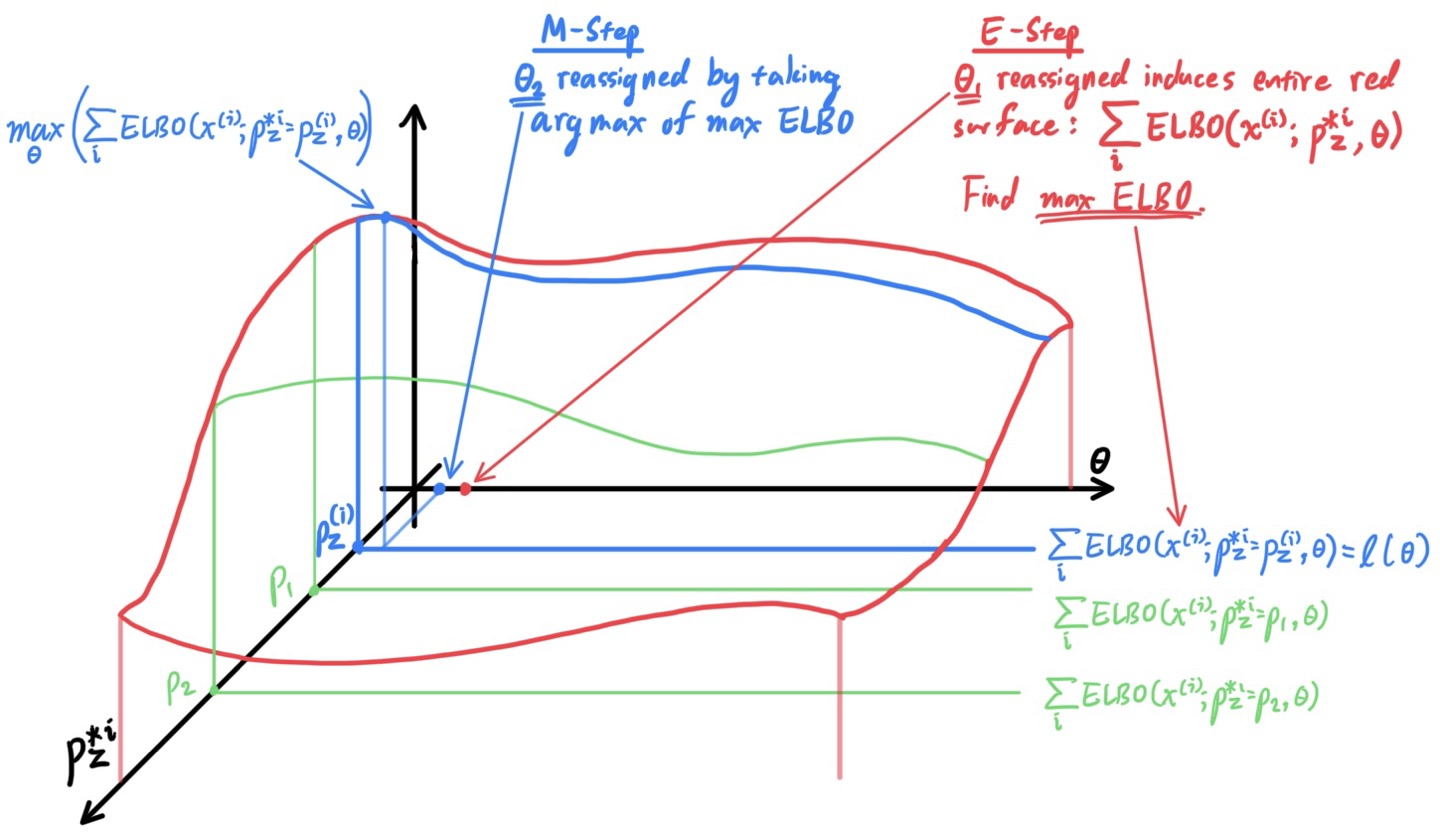
\includegraphics[width=0.7\textwidth]{img/EM_second_iteration.jpg}
    \caption{} 
    \label{fig:EM_second_iteration}
  \end{figure}

  \begin{definition}[EM Algorithm for General Estimation Problems]
    Given a training set $\{x^{(i)}\}_{i=1}^n \in \mathbb{R}^d$, let us assume that the random variable $X$ that these examples follow can be modeled by specifying a joint distribution of a multinomial and some arbitrary distributions. Let there be $k$ clusters, and let 
    \begin{itemize}
      \item $Z$ be the multinomial distribution representing which Gaussian cluster each example $x$ falls in, with density $p_Z (j)$ and represented by vector $\phi \in \mathbb{R}^k$ so that $\mathbb{P}(Z = j) = \phi_j$. Let the parameters of $\phi$ be encoded in $\theta$.
      \item The set of conditional distributions
        \[X\,|\,Z = j \sim X_j \text{ for } j = 1, 2, \ldots, k\]
      are arbitrary distributions with some parameters, also all encoded in $\theta$.  
    \end{itemize}

    The EM algorithm is described as such: 
    \begin{enumerate}
      \item Initialize $\theta$.
      \item \textbf{(E Step)} Since $l(\theta)$ is bounded below for all $p_Z^{*1}, \ldots, p_Z^{*n}$ as 
        \[l(\theta) \equiv \sum_{i=1}^n \log p\big( x^{(i)}; \, \theta\big) \geq \sum_{i=1}^n \text{ELBO}\big( x^{(i)}; \, p_Z^{*i}, \theta\big)\]
      setting $p_Z^{*i} (j) = p_Z^{(i)} (j) = p_Z \big(j\,|\, x^{(i)}; \, \theta\big)$ for all $i = 1, \ldots, n$ would put $l$ into a new form for these specific fixed values of $p_Z^{*i}$. 
        \[l(\theta) = \sum_{i=1}^n \text{ELBO}\big(x^{(i)}; p_Z^{(i)}, \theta \big)\]
      \item \textbf{(M Step)} We maximize this equivalent form of $l(\theta)$ with respect to $\theta$ whilst fixing the choice of $p_Z^{(i)}$. That is, we set the value of $\theta$ as 
      \begin{align*}  
        \theta & = \text{arg}\; \max_\theta \sum_{i=1}^n \text{ELBO} \big( x^{(i)}; \, p_Z^{(i)}, \theta \big) \\
        & = \text{arg}\; \max_\theta \sum_{i=1}^n \sum_{j=1}^k p_Z^{(i)} (j)\; \log \bigg( \frac{p(x^{(i)}, Z = j; \, \theta)}{p_Z^{(i)} (j)} \bigg) \\
        & = \text{arg}\; \max_\theta \sum_{i=1}^n \sum_{j = 1}^k p_Z \big(j\,|\, x^{(i)}; \, \theta \big)\, \log \bigg( \frac{p(x^{(i)}, Z = j; \, \theta)}{p_Z \big(j\,|\, x^{(i)}; \, \theta \big)} \bigg)
      \end{align*}
      \item We have successfully updated $\theta$. Now, we repeat steps 2 and 3 until convergence. Step 2 can bring improvements because we have changed the $\theta$, which means that there is a new sum of ELBO functions of the $\theta$ that serves as a new lower bound.
    \end{enumerate}
  \end{definition}

\subsection{Gaussian Mixture Models}

  Given a training set ${\mathbf{x}^{(i)}}_{i=1}^n$ (without the $y$-labels and so in the unsupervised setting), there are some cases where it may seem like we can fit multiple Gaussian distributions in the input space $\mathcal{X}$. For example, the points below seem like they can be fitted well with 3 Gaussians.

  \begin{figure}[H]
    \centering
    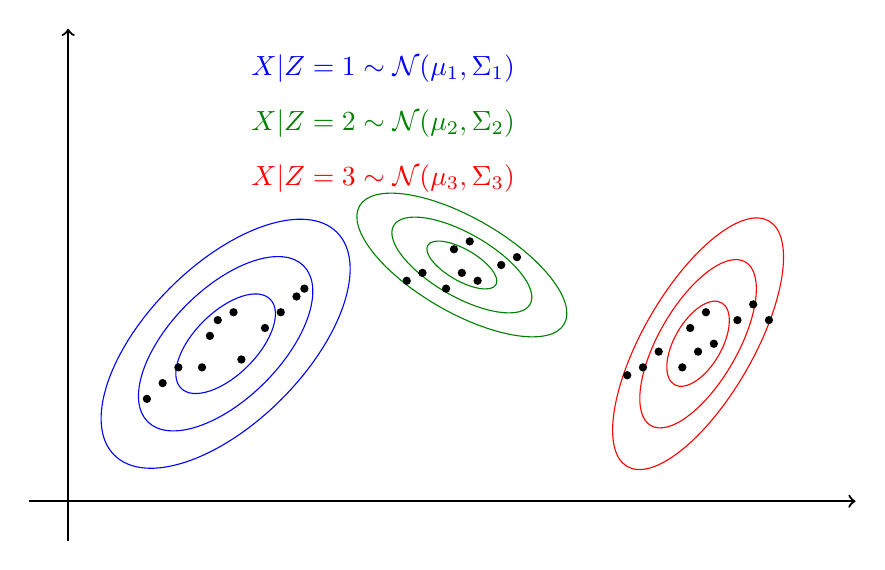
\begin{tikzpicture}
      % Draw axes
      \draw[black, ->, line width=0.8pt] (-0.5,0) -- (10,0);
      \draw[black, ->, line width=0.8pt] (0,-0.5) -- (0,6);
      
      % Equations at top
      \node[blue] at (4,5.5) {$X|Z=1 \sim \mathcal{N}(\mu_1, \Sigma_1)$};
      \node[green!50!black] at (4,4.8) {$X|Z=2 \sim \mathcal{N}(\mu_2, \Sigma_2)$};
      \node[red] at (4,4.1) {$X|Z=3 \sim \mathcal{N}(\mu_3, \Sigma_3)$};
      
      % First Gaussian (blue)
      \draw[blue, rotate around={45:(2,2)}] (2,2) ellipse (2 and 1);
      \draw[blue, rotate around={45:(2,2)}] (2,2) ellipse (1.4 and 0.7);
      \draw[blue, rotate around={45:(2,2)}] (2,2) ellipse (0.8 and 0.4);
      
      % Blue cluster points - more spread out
      \fill[black] (1.7,1.7) circle (1.5pt);
      \fill[black] (1.8,2.1) circle (1.5pt);
      \fill[black] (2.1,2.4) circle (1.5pt);
      \fill[black] (2.2,1.8) circle (1.5pt);
      \fill[black] (1.9,2.3) circle (1.5pt);
      \fill[black] (1.4,1.7) circle (1.5pt);
      \fill[black] (2.5,2.2) circle (1.5pt);
      \fill[black] (2.7,2.4) circle (1.5pt);
      \fill[black] (1.2,1.5) circle (1.5pt);
      \fill[black] (2.9,2.6) circle (1.5pt);
      \fill[black] (3.0,2.7) circle (1.5pt);
      \fill[black] (1.0,1.3) circle (1.5pt);
      
      % Second Gaussian (green)
      \draw[green!50!black, rotate around={-30:(5,3)}] (5,3) ellipse (1.5 and 0.6);
      \draw[green!50!black, rotate around={-30:(5,3)}] (5,3) ellipse (1 and 0.4);
      \draw[green!50!black, rotate around={-30:(5,3)}] (5,3) ellipse (0.5 and 0.2);
      
      % Green cluster points - more oval shaped
      \fill[black] (4.8,2.7) circle (1.5pt);
      \fill[black] (4.9,3.2) circle (1.5pt);
      \fill[black] (5.0,2.9) circle (1.5pt);
      \fill[black] (5.1,3.3) circle (1.5pt);
      \fill[black] (5.2,2.8) circle (1.5pt);
      \fill[black] (4.5,2.9) circle (1.5pt);
      \fill[black] (5.5,3.0) circle (1.5pt);
      \fill[black] (4.3,2.8) circle (1.5pt);
      \fill[black] (5.7,3.1) circle (1.5pt);
      
      % Third Gaussian (red)
      \draw[red, rotate around={60:(8,2)}] (8,2) ellipse (1.8 and 0.7);
      \draw[red, rotate around={60:(8,2)}] (8,2) ellipse (1.2 and 0.5);
      \draw[red, rotate around={60:(8,2)}] (8,2) ellipse (0.6 and 0.3);
      
      % Red cluster points - more spread out
      \fill[black] (7.8,1.7) circle (1.5pt);
      \fill[black] (7.9,2.2) circle (1.5pt);
      \fill[black] (8.0,1.9) circle (1.5pt);
      \fill[black] (8.1,2.4) circle (1.5pt);
      \fill[black] (8.2,2.0) circle (1.5pt);
      \fill[black] (7.5,1.9) circle (1.5pt);
      \fill[black] (8.5,2.3) circle (1.5pt);
      \fill[black] (7.3,1.7) circle (1.5pt);
      \fill[black] (8.7,2.5) circle (1.5pt);
      \fill[black] (8.9,2.3) circle (1.5pt);
      \fill[black] (7.1,1.6) circle (1.5pt);
    \end{tikzpicture}
    \caption{Example of data that can be fitted with 3 Gaussians}
  \end{figure}

  Therefore, we can construct a best-fit model as a composition of a multinomial distribution (to decide which one of the Gaussians $\mathbf{x}$ should follow) followed by a Gaussian. That is, to find the distribution of $\mathbf{x}$ and get the density function $p(\mathbf{x})$, we condition it on the random variable $Z$. More specifically, we let
  \begin{equation}
    Z \sim \text{Multinomial}(\boldsymbol{\phi}), \;\;\;\;\; \boldsymbol{\phi} = \begin{pmatrix} \phi_1 \ \phi_2 \ \ldots \ \phi_k \end{pmatrix} \text{ such that } \sum_{i=1}^k \phi_i = 1
  \end{equation}
  and define the conditional distributions as
  \begin{align*}
    \mathbf{X} \mid Z = 1 & \sim \mathcal{N}(\boldsymbol{\mu}_1, \boldsymbol{\Sigma}_1) \\
    \mathbf{X} \mid Z = 2 & \sim \mathcal{N}(\boldsymbol{\mu}_2, \boldsymbol{\Sigma}_2) \\
    \ldots & \sim \ldots \\
    \mathbf{X} \mid Z = j & \sim \mathcal{N}(\boldsymbol{\mu}_j, \boldsymbol{\Sigma}_j) \\
    \ldots & \sim \ldots \\
    \mathbf{X} \mid Z = k & \sim \mathcal{N}(\boldsymbol{\mu}_k, \boldsymbol{\Sigma}_k)
  \end{align*}
  Therefore, our model says that each $\mathbf{x}^{(i)}$ was generated by randomly choosing $z^{(i)}$ from ${1, \ldots, k}$ according to some multinomial, and then the $\mathbf{x}^{(i)}$ was drawn from one of the $k$ Gaussians depending on $z^{(i)}$. This model is called the \textbf{mixture of Gaussians model}. The parameters of our model are: 

  \begin{itemize}
    \item The vector $\boldsymbol{\phi} \in \mathbb{R}^k$ (which really has $k-1$ parameters) characterizing the multinomial distribution.
    \item The set of vectors $\boldsymbol{\mu}_1, \boldsymbol{\mu}_2, \ldots, \boldsymbol{\mu}_k$ representing the mean vectors of each multivariate Gaussian. For simplicity, we'll denote this set of vectors as $\bm{\mu}$.
    \item The set of symmetric, positive-definite matrices $\boldsymbol{\Sigma}_1, \boldsymbol{\Sigma}_2, \ldots, \boldsymbol{\Sigma}_k$ representing the covariance matrices of each multivariate Gaussian. For simplicity, we'll denote this set of matrices as $\bm{\Sigma}$.
  \end{itemize}

  We can write down the log-likelihood of the given data $\mathbf{x}^{(i)}$'s as a function of all the parameters above as:

  \begin{align*}
    l (\boldsymbol{\phi}, \bm{\mu}, \bm{\Sigma}) & = \sum_{i=1}^n \log, p\big( \mathbf{x}^{(i)} ;  \boldsymbol{\phi}, \bm{\mu}, \bm{\Sigma} \big) \\
    & = \sum_{i=1}^n \log \bigg( \sum_{j=1}^k  p\big( \mathbf{x}^{(i)} \mid z^{(i)} = j ; \bm{\mu}, \bm{\Sigma} \big) , p\big( z^{(i)} = j; \boldsymbol{\phi}\big) \bigg)
  \end{align*}

  This equation above tells us the (log-) likelihood of the data landing on the $\mathbf{x}^{(i)}$'s given that we have parameters $\boldsymbol{\phi}, \bm{\mu}, \bm{\Sigma}$. Note that since we only know that the \textit{final} value of the $i$th sample is $\mathbf{x}^{(i)}$ and not anything at all about which value $z^{(i)}$ the $i$th sample had, there is an extra unknown in this model. That is, we do not know which one of the $k$ Gaussians the $\mathbf{x}^{(i)}$ was generated from. These values $z^{(i)}$ are called the \textbf{hidden/latent variables}.

  If we did know the values of the hidden variables $z^{(i)}$ (i.e. if we knew which of the $k$ Gaussians each $\mathbf{x}^{(i)}$ was generated from), then our log likelihood function would be much more simple since now, our givens will be both $\mathbf{x}^{(i)}$ \textit{and} $z^{(i)}$. Therefore, we don't have to condition on the $z^{(i)}$ and can directly calculate the log of the probability of us having sample values $(z^{(1)}, \mathbf{x}^{(1)}), (z^{(2)}, \mathbf{x}^{(2)}), \ldots, (z^{(n)}, \mathbf{x}^{(n)})$.

  \begin{align*}
    l(\boldsymbol{\phi}, \bm{\mu}, \bm{\Sigma}) & = \sum_{i=1}^n \log , p\big( \mathbf{x}^{(i)}; \boldsymbol{\phi}, \bm{\mu} ,\bm{\Sigma}\big) \\
    & = \sum_{i=1}^n \log, p\big( \mathbf{x}^{(i)}, z^{(i)}; \boldsymbol{\phi}, \bm{\mu} ,\bm{\Sigma}\big) \\
    & = \sum_{i=1}^n \log, p\big( \mathbf{x}^{(i)} \mid z^{(i)}; \bm{\mu}, \bm{\Sigma}) \; p\big( z^{(i)}; \boldsymbol{\phi} \big)
  \end{align*}

  This model, with known $z^{(i)}$'s, is basically the GDA model, which is easy to calculate. That is, the maximum values of $\boldsymbol{\phi}, \bm{\mu}, \bm{\Sigma}$ are:

  \begin{align*}
    \phi_j & = \frac{1}{n} \sum_{i=1}^n \mathbbm{1}_{z^{(i)} = j} \\
    \boldsymbol{\mu}_j & = \frac{\sum_{i=1}^n \mathbbm{1}_{z^{(i)} = j} \mathbf{x}^{(i)}}{\sum_{i=1}^n \mathbbm{1}_{z^{(i)} = j}} \\
    \boldsymbol{\Sigma}_j & = \frac{1}{\sum_{i=1}^n \mathbbm{1}_{z^{(i)} = j}} \sum_{i=1}^n \mathbbm{1}_{z^{(i)}} \big( \mathbf{x}^{(i)} - \boldsymbol{\mu}_j \big),\big(\mathbf{x}^{(i)} - \boldsymbol{\mu}_j \big)^T
  \end{align*}

  for $j = 1, \ldots, d$. But since we do \textit{not} know the values of $z^{(i)}$, we first try to "guess" the values of the $z^{(i)}$'s and then update the parameters of our model assuming our guesses are correct. Let us clarify some notation:

  \begin{itemize}
    \item The distribution that we will iteratively reassign over and over again is $Z$, with density $p_Z (z)$ that maps $z \mapsto \phi_z$, where $\boldsymbol{\phi}$ is a vector that represents the density. The algorithm will initialize $p_Z$ and have it converge to the true multinomial density. Note that $Z$ in this context could represent the true multinomial distribution $Z$ or could represent the distributions iteratively produced by the algorithm that should converge onto the true $Z$ (usually the latter).

    \item The $k$ Gaussian distributions that we will iteratively reassign over and over again is $\mathcal{N}_1, \mathcal{N}_2, \ldots, \mathcal{N}k$, with densities $p_{\mathcal{N}1}(\mathbf{x}), \ldots, p_{\mathcal{N}k}(\mathbf{x})$ that maps $\mathbf{x} \mapsto p_{\mathcal{N}j}(\mathbf{x})$.

    \item The distribution of the entire random variable $\mathbf{X}$ will have density $p_X(\mathbf{x})$. Since we are iteratively reassigning the densities $p_Z$ and $p{\mathcal{N}_j}$, this joint distribution of $\mathbf{X}$ will also get modified.
  \end{itemize}

  \begin{definition}[EM Algorithm]
    The \textbf{Expectation-Maximization (EM) Algorithm} has the following steps:

    \begin{enumerate}
      \item We initialize our values of $\theta$, which can be chosen randomly or by \textbf{K-means initialization} (not explained here).
      \begin{itemize}
        \item We can randomly assign our values of $\mu_j$'s and the $\Sigma_j$'s in $\mathbb{R}^d$.
        \item We can randomly assign the density of our guess multinomial $p_Z(z)$, represented by vector
        \[\phi = \begin{pmatrix} \phi_1 \\ \vdots \\ \phi_k \end{pmatrix} \text{ with } \sum_{j=1}^k \phi_j = 1\]
        where $p_Z(z) \equiv \phi_z$ for $z = 1, \ldots, k$.
      \end{itemize}

      \item \textbf{(E Step)} Now that we have our prior guess of what $Z$ and its density function $p_Z$ is, we can calculate its posterior density function by taking one observed example $x^{(i)}$ and modifying $p_Z$ to $p_Z^{(i)}$. This superscript $(i)$ on the distribution $p_Z$ indicates that this is a posterior density created from observing $x^{(i)}$. (The motivation for this construction is explained more specifically in the next section involving Jensen's inequality.) Using Bayes' rule, we should calculate $n$ density functions
      \[p_Z^{(i)}(z) \equiv p_Z(z\,|\,x^{(i)}; \phi, \mathbf{\mu}, \mathbf{\Sigma}) \text{ for } i = 1, \ldots, n\]
      For easier notation, we let $\phi^{(i)}$ be the vector representation of the density $p_Z^{(i)}$. That is,
      \[\phi^{(i)} = \begin{pmatrix} \phi_1^{(i)} \\ \vdots \\ \phi_k^{(i)} \end{pmatrix} \text{ with } \sum_{j=1}^k \phi_j^{(i)} = 1\]
      where $p_Z^{(i)}(z) \equiv \phi^{(i)}_z$ for $z = 1, \ldots, k$ and $0$ otherwise. Then, we can calculate $\phi^{(i)}$ (and therefore $p_Z^{(i)}$) component-wise by calculating each $\phi_j^{(i)}$ (which is the probability of a point being in the $j$th cluster, given that we observe example $x^{(i)}$):
      \begin{align*}
          \phi_j^{(i)} &= p_Z^{(i)}\big(z = j;\, \phi, \mathbf{\mu}, \mathbf{\Sigma}\big) \\
          &= p_Z\big(z = j\,|\,x^{(i)};\,\phi, \mathbf{\mu}, \mathbf{\Sigma}\big) \\
          &= \frac{p_{\mathcal{N}_j}\big(x^{(i)}\,|\,z^{(i)} = j;\,\mathbf{\mu}, \mathbf{\Sigma}\big) \; p_Z\big(z^{(i)} = j;\,\phi\big)}{p_X\big(x^{(i)};\,\phi, \mathbf{\mu}, \mathbf{\Sigma}\big)} \\
          &= \frac{p_{\mathcal{N}_j}\big(x^{(i)}\,|\,z^{(i)} = j;\,\mathbf{\mu}, \mathbf{\Sigma}\big) \; p_Z\big(z^{(i)} = j;\,\phi\big)}{\sum_{l=1}^k p_{\mathcal{N}_j}\big(x^{(i)}\,|\,z^{(i)} = l;\,\mathbf{\mu}, \mathbf{\Sigma}\big)\; p_Z\big(z^{(i)} = l;\,\phi\big)}
      \end{align*}
      Note that we have everything we need to calculate the posterior probability distribution $p_Z^{(i)}(z)$ of a point being in any cluster.
      \begin{itemize}
          \item $p_{\mathcal{N}_j}(x^{(i)}\,|\,z^{(i)} = j)$ represents the conditional Gaussian density, which is completely defined because the parameters $\mu_j, \Sigma_j$ are already defined in initialization.
          \item $p_Z(z^{(i)} = j; \phi)$ is really just the probability $\phi_j$ that a given point is in the $j$th cluster, which we've also defined in initialization.
          \item $p_X(x^{(i)})$ represents the distribution of the entire random variable $X$ of the entire training set. Knowing the first two and taking the sum gives this density function $p_X$.
      \end{itemize}
      Therefore, we should end up with $n$ different $k$-vectors $\phi^{(1)}, \phi^{(2)}, \ldots, \phi^{(n)}$, each representing our best guess of what multinomial density $p_Z^{(i)}$ each $x^{(i)}$ had followed in order to be at the given points.


      \begin{figure}[H]
        \centering
        \begin{subfigure}[b]{0.48\textwidth}
          \centering
          \begin{tikzpicture}[scale=1.]
            \draw[->] (-0.5,0) -- (5,0);
            \draw[->] (0,-0.5) -- (0,3.5);
            
            % Points and labels
            \fill[red] (1,1) circle (3pt);
            \fill[red] (1.5,0.8) circle (3pt);
            \fill[red] (2,1.5) circle (3pt);
            \node[red] at (3,1.5) {$\phi_1=\frac{3}{6}$};
            
            \fill[blue] (3,2.5) circle (3pt);
            \fill[blue] (3.2,2) circle (3pt);
            \node[blue] at (4,2.5) {$\phi_2=\frac{2}{6}$};
            
            \fill[green!50!black] (4,1) circle (3pt);
            \node[green!50!black] at (4.5,1) {$\phi_3=\frac{1}{6}$};
          \end{tikzpicture}
          \caption{Hard label assignments.}
          \label{fig:hard-guesses}
        \end{subfigure}
        \hfill 
        \begin{subfigure}[b]{0.48\textwidth}
          \centering
          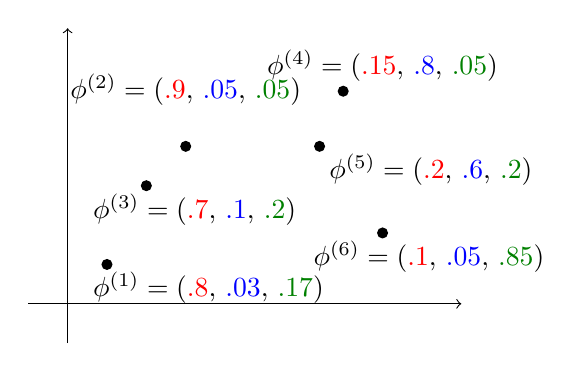
\begin{tikzpicture}[scale=1]
            \draw[->] (-0.5,0) -- (5,0);
            \draw[->] (0,-0.5) -- (0,3.5);
            
            % Points and colored vectors
            \fill (0.5,0.5) circle (2pt);
            \node[right] at (0.2,0.2) {$\phi^{(1)} = ($\textcolor{red}{.8}, \textcolor{blue}{.03}, \textcolor{green!50!black}{.17}$)$};
            
            \fill (1.5,2) circle (2pt);
            \node[above] at (1.5,2.4) {$\phi^{(2)} = ($\textcolor{red}{.9}, \textcolor{blue}{.05}, \textcolor{green!50!black}{.05}$)$};
            
            \fill (1,1.5) circle (2pt);
            \node[right] at (0.2,1.2) {$\phi^{(3)} = ($\textcolor{red}{.7}, \textcolor{blue}{.1}, \textcolor{green!50!black}{.2}$)$};
            
            \fill (3.5,2.7) circle (2pt);
            \node[above] at (4,2.7) {$\phi^{(4)} = ($\textcolor{red}{.15}, \textcolor{blue}{.8}, \textcolor{green!50!black}{.05}$)$};
            
            \fill (3.2,2) circle (2pt);
            \node[right] at (3.2,1.7) {$\phi^{(5)} = ($\textcolor{red}{.2}, \textcolor{blue}{.6}, \textcolor{green!50!black}{.2}$)$};
            
            \fill (4,0.9) circle (2pt);
            \node[right] at (3,0.6) {$\phi^{(6)} = ($\textcolor{red}{.1}, \textcolor{blue}{.05}, \textcolor{green!50!black}{.85}$)$};
          \end{tikzpicture}
          \caption{Soft probability assignments.}
          \label{fig:soft-guesses}
        \end{subfigure}
        \caption{Let us elaborate further on the intuition of this step. In the normal GDA with given values of $z^{(i)}$, we have $\phi_j = \frac{1}{n} \sum_{i=1}^n 1\{z^{(i)} = j\} = \frac{1}{n}\big(\text{Number of Samples in }j\text{th Gaussian}\big)$, which is a sum of "hard" guesses, meaning that each $x^{(i)}$ is undoubtedly in cluster $j$ or not, and so to find out our best guess for the true vector $\phi$, all we have to do is find out the proportion of all examples in each of the $k$ groups and we're done (without needing to iterate). However, in our EM model, we do not know the $z^{(i)}$'s, and so the best we can do is give the \textit{probability} $\phi^{(i)}_j$ that $x^{(i)}$ is in cluster $j$. So for each point $x^{(i)}$, the model has changed from it being undoubtedly in group $z^{(i)} = j$ to it having a probability of being in $\phi^{(i)}_j$ for $j = 1, \ldots, k$.}
        \label{fig:guesses-comparison}
      \end{figure}

      \item \textbf{(M Step)} With these $n$ separate posterior estimates of $Z$ for each observation $x^{(i)}$, we can simply average all of them and say that our best estimate of $\phi$ is
      \[\phi = \frac{1}{n} \sum_{i=1}^n \phi^{(i)}\]
      We can interpret the vectors $\phi^{(i)}$ as tuples where $\phi^{(i)}_j$ describes the expected "portion" of each sample $x^{(i)}$ to be in group $j$. So, we are adding up all the "portions" of the points that are expected to be in cluster $j$ to get $\phi_j = \sum_{i=1}^n \phi_j^{(i)}$.

      Now, given the $j$th Gaussian cluster, we would like to compute its mean $\mu_j$. Since each $x^{(i)}$ has probability $\phi^{(i)}_j$ of being in cluster $j$, we can weigh each of the $n$ points by $\phi^{(i)}_j$ (which determines how "relevant" $x^{(i)}$ is to cluster $j$) and average these (already weighted) points to get our "best-guess" of the mean $\mu_j$.
      \[\mu_j = \frac{\sum_{i=1}^n \phi^{(i)}_j x^{(i)}}{\sum_{i=1}^n \phi_j^{(i)}}\]

      \begin{figure}[H]
        \centering 
        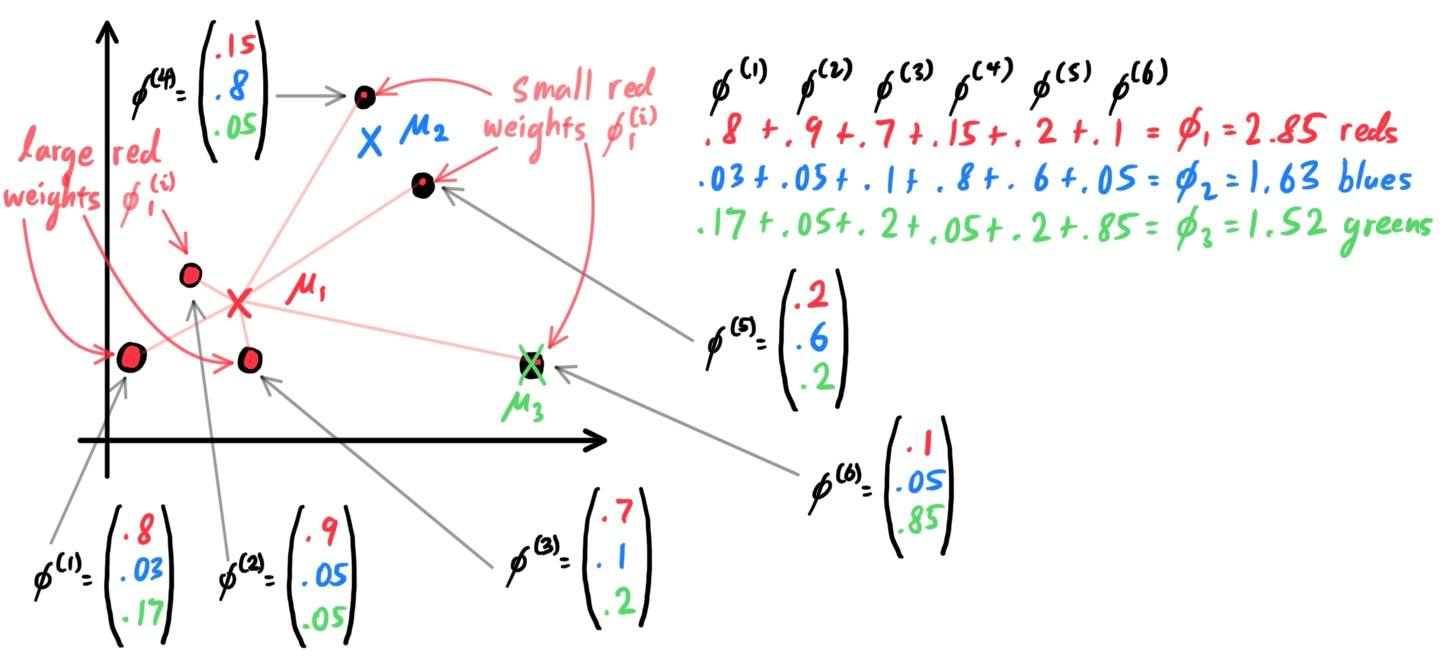
\includegraphics[scale=0.27]{img/weighted_means.jpg}
        \caption{} 
        \label{fig:weighted_means}
      \end{figure}

      With this logic of weighted points, we finally update the covariance matrices $\Sigma_j$ as below:
      \[\Sigma_j = \frac{1}{\sum_{i=1}^n \phi_j^{(i)}} \sum_{i=1}^n \phi^{(i)}_j \,\big(x^{(i)} - \mu_j\big)\big(x^{(i)} - \mu_j\big)^T\]

      \item Now, we have new values of $\phi, \mu_1, \ldots, \mu_k, \Sigma_1, \ldots, \Sigma_k$ that we can work with. With these new values, repeat steps 2 and 3 until convergence.
    \end{enumerate}
  \end{definition}

  In summary, this entire algorithm results from modifying the "hard" data of each point $x^{(i)}$ being undoubtedly in one cluster to a model containing points $x^{(i)}$ that have been "smeared" around different clusters, with a probability $\phi_j^{(i)}$ being in cluster $j$. 

  \begin{definition}[Mixture of Gaussians Algorithm: Summary]
    Given a training set $\{x^{(i)}\}_{i=1}^n \in \mathbb{R}^d$, let us assume that the random variable $X$ that these examples follow can be modeled by specifying a joint distribution of a multinomial and Gaussians. 
    That is, it follows a Gaussian mixture model (GMM) of $k$ Gaussian clusters. Let
    \begin{itemize}
      \item $Z$ be the multinomial distribution representing which Gaussian cluster each example $x$ falls in, with density represented by vector $\phi \in \mathbb{R}^k$ so that $\mathbb{P}(Z = j) \equiv \phi_j$.
      \item The set of conditional distributions 
        \[X\,|\,Z = j \sim \mathcal{N}(\mu_j, \Sigma_j) \text{ for } j = 1, 2, \ldots, k\]
      are multivariate Gaussian, with mean vectors $\mu_1, \ldots, \mu_k$ and covariance matrices $\Sigma_1, \ldots, \Sigma_k$. 
    \end{itemize}
    Let all the parameters be denoted as $\theta$. Then, the EM algorithm is as such: 
    \begin{enumerate}
      \item Initialize the multinomial vector $\phi$, the $\mu_j$'s, and the $\Sigma_j$'s.
      \item \textbf{(E Step)} Calculate the $n$ vectors
        \[\phi^{(i)} = \begin{pmatrix} \phi_1^{(i)} \\ \vdots \\ \phi_k^{(i)} \end{pmatrix} \text{ for all } i = 1, \ldots, n\]
      that represent the posterior distribution of $Z$ given observed $x^{(i)}$ by computing 
        \begin{align*} 
          \phi_j^{(i)} & = p_Z^{(i)} \big(z = j;\, \phi, \mathbf{\mu}, \mathbf{\Sigma} \big) \\
          & = p_Z \big(z = j\,|\, x^{(i)}; \, \phi, \mathbf{\mu}, \mathbf{\Sigma} \big) \\
          & = \frac{p_{\mathcal{N}_j} \big(x^{(i)}\,|\,z^{(i)} = j; \, \mathbf{\mu}, \mathbf{\Sigma}\big) \; p_Z \big(z^{(i)} = j;\, \phi \big)}{p_X \big(x^{(i)};\, \phi, \mathbf{\mu}, \mathbf{\Sigma}\big)} \\
          & = \frac{p_{\mathcal{N}_j} \big(x^{(i)}\,|\,z^{(i)} = j; \, \mathbf{\mu}, \mathbf{\Sigma}\big) \; p_Z \big(z^{(i)} = j;\, \phi \big)}{\sum_{l=1}^k p_{\mathcal{N}_j} \big( x^{(i)}\,|\, z^{(i)} = l;\, \mathbf{\mu}, \mathbf{\Sigma} \big)\; p_Z \big(z^{(i)} = l; \,\phi\big)}
        \end{align*}
      \item \textbf{(M Step)} Reassign the value of $\theta$ as 
        \begin{align*} 
          \phi & = \frac{1}{n} \sum_{i=1}^n \phi^{(i)} \\
          \mu_j & = \frac{\sum_{i=1}^n \phi_j^{(i)} x^{(i)}}{\sum_{i=1}^n w_j^{(i)}} \text{ for } j = 1, \ldots, n \\
          \Sigma_j & = \frac{1}{\sum_{i=1}^n \phi_j^{(i)}} \sum_{i=1}^n \phi^{(i)}_j \, \big(x^{(i)} - \mu_j \big) \big(x^{(i)} - \mu_j\big)^T \text{ for } j = 1, \ldots, n 
        \end{align*}
      \item Repeat steps 2 and 3 until convergence.
    \end{enumerate}
  \end{definition}

\subsection{Nonlinear ICA} 
